\section{Vorgehen}

\begin{frame}
  \frametitle{Programmaufbau}
\end{frame}
 
 
 
 
 

\begin{frame}
\frametitle{Inverse Kinematik - Einführung}
\textit{Wie muss die Winkelstellung des Greifarms sein, damit die aktuelle Position der Hand erreicht wird?}\\
\vspace*{1cm}
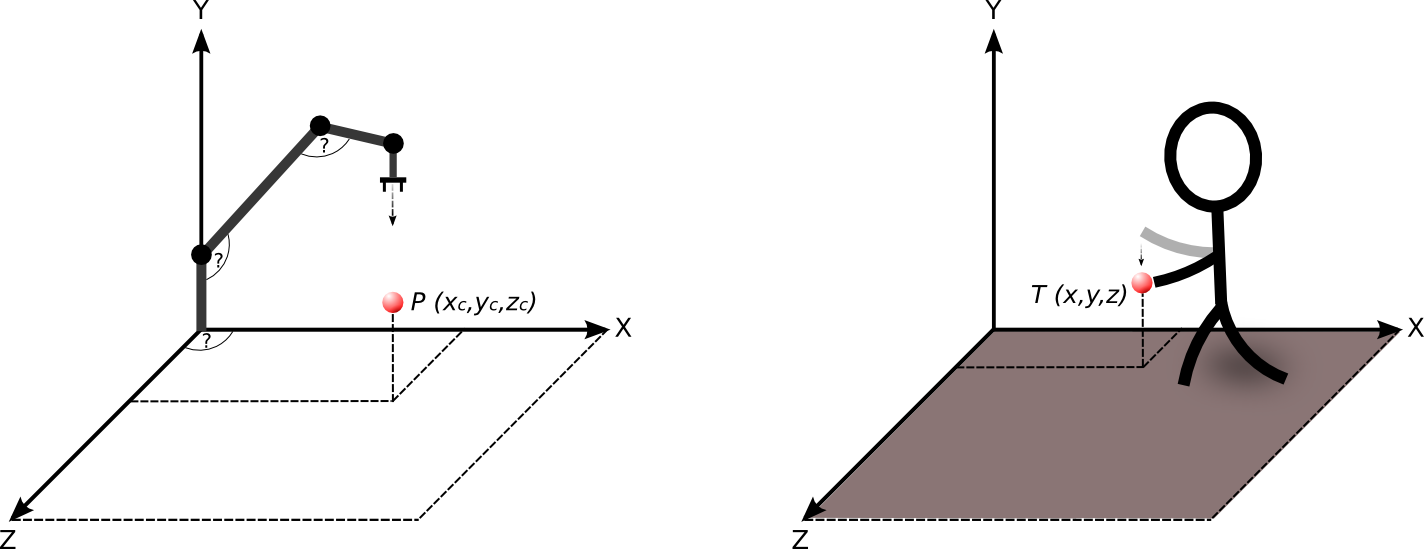
\includegraphics[width=\textwidth]{imgs/kinematikProblem.png}
\end{frame}

\begin{frame}
\frametitle{Inverse Kinematik - Vorgehen}
\begin{columns}
\begin{column}{.48\textwidth}
\begin{enumerate}
\item Aktuelle 3D Position auslesen.
\item Iterativ alle Winkel berechnen.
\item Servostellungen aktualisieren.
\item Wiederhole 1-3.
\end{enumerate}
\end{column}%
\hfill%
\begin{column}{.48\textwidth}
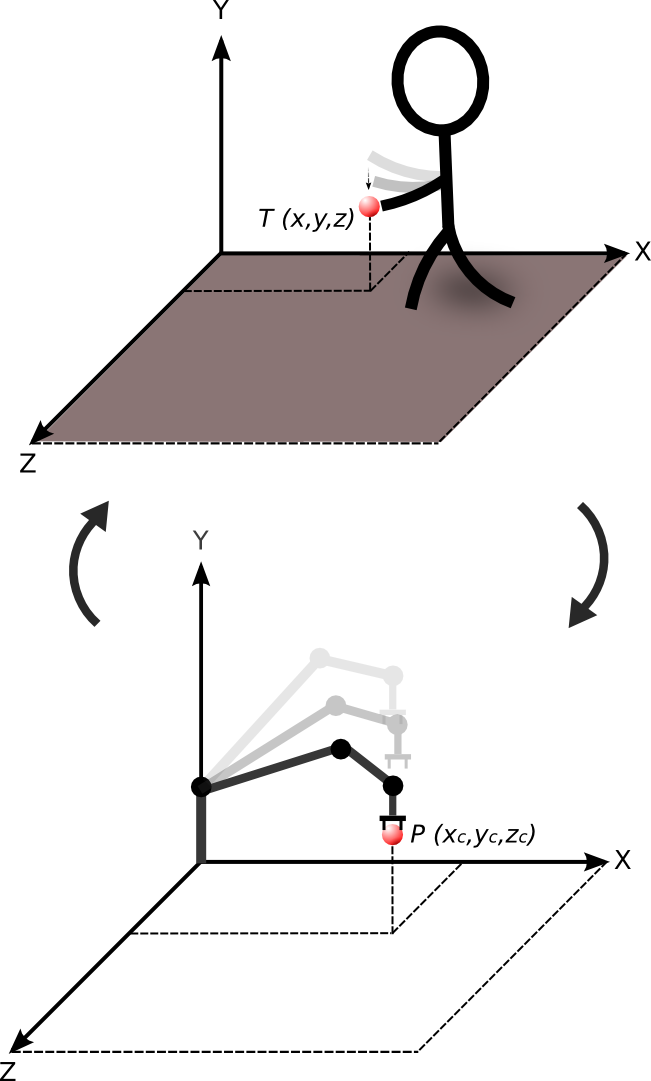
\includegraphics[scale=0.248]{imgs/kinematikCycle.png}
\end{column}
\end{columns}
\end{frame}

\begin{frame}
\frametitle{Inverse Kinematik - Geometrische Lösung}
\begin{block}{Grundlage: Kosinussatz}
\begin{columns}
\begin{column}{.3\textwidth}
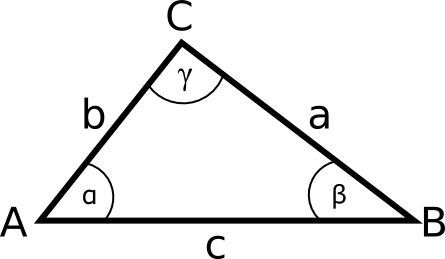
\includegraphics[scale=0.25]{imgs/cos.png}
\end{column}%
\begin{column}{.5\textwidth}
$c^2 = a^2 + b^2 - 2ab * \cos	\gamma$
\end{column}
\end{columns}
\end{block}

\begin{columns}
\begin{column}{.48\textwidth}
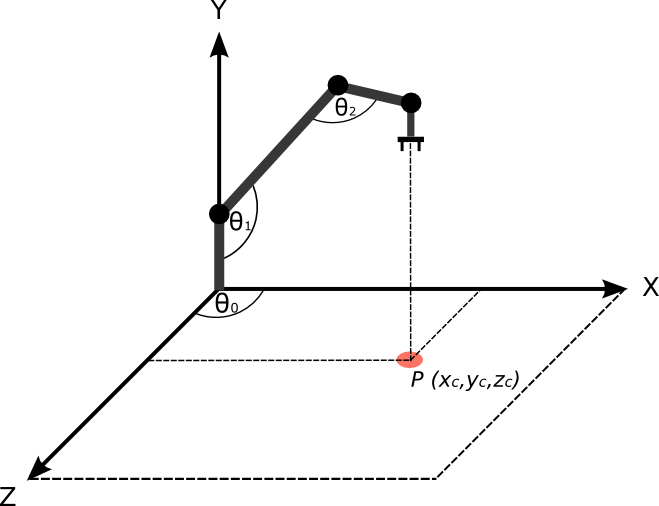
\includegraphics[scale=0.248]{imgs/3d_robo.png}
\end{column}%
\hfill%
\begin{column}{.48\textwidth}
\textbf{Rotation: Winkel $\theta_0$}
\begin{eqnarray*}
	\theta_0 = atan2(z_c, x_c) \left[+ \pi \right]
	\end{eqnarray*}
\end{column}
\end{columns}

\end{frame}

\begin{frame}
\frametitle{Inverse Kinematik - Geometrische Lösung}
\begin{columns}
\begin{column}{.32\textwidth}
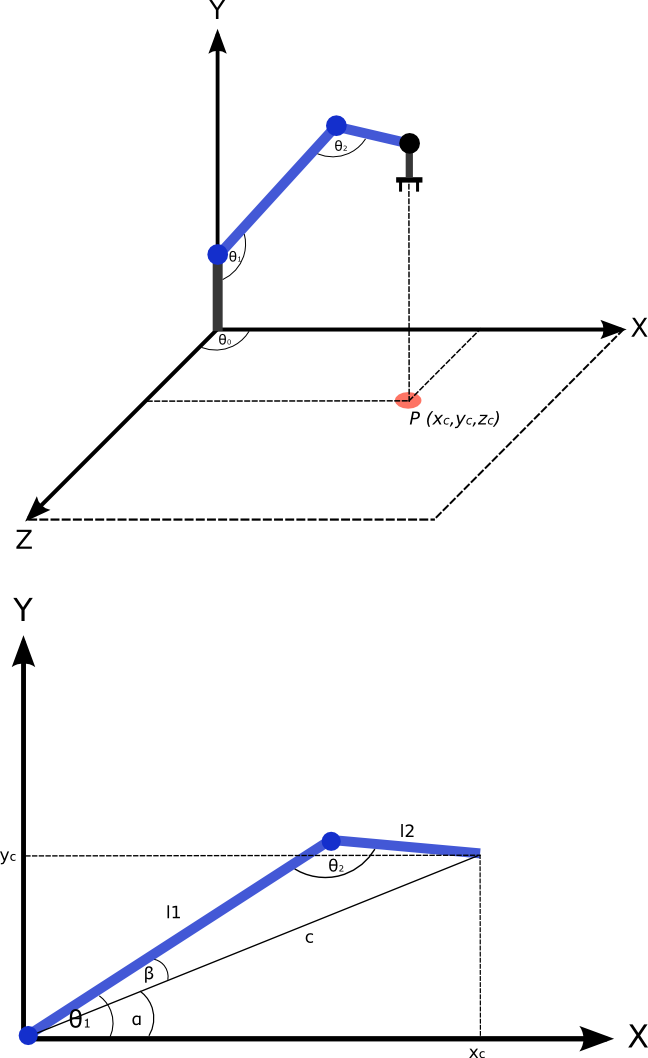
\includegraphics[scale=0.2]{imgs/inverseKinematik.png}
\end{column}%
\begin{column}{.72\textwidth}
\textbf{Beugung: Winkel $\theta_1$}
\small \begin{eqnarray*}
\theta_1 &=& \alpha + \beta \\
\theta_1 &=& atan2(y_c, z_c) + atan2(E, \pm \sqrt{1-E^2}) \\ \\
\cos \beta &=& \frac{l_1^2 + y_c^2 + z_c^2 - l_2^2}{2*l_1*\sqrt{z_c^2 + y_c^2}} := E 
\end{eqnarray*}
\end{column}
\end{columns}
\end{frame}

\begin{frame}
\frametitle{Inverse Kinematik - Geometrische Lösung}
\begin{columns}
\begin{column}{.32\textwidth}
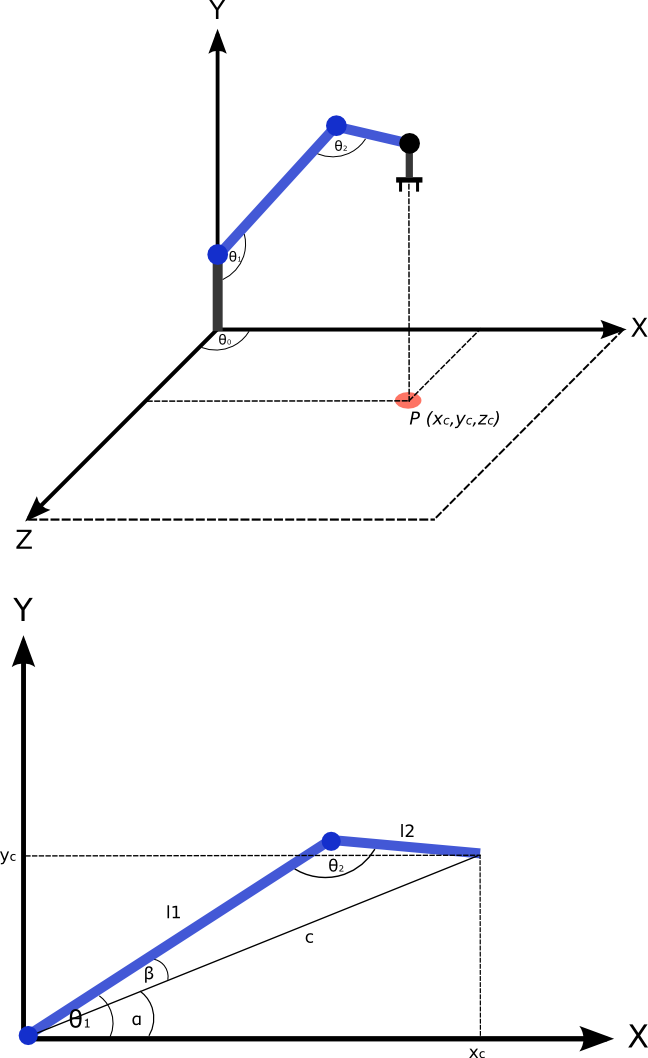
\includegraphics[scale=0.2]{imgs/inverseKinematik.png}
\end{column}%
\hfill
\begin{column}{.72\textwidth}
\textbf{Beugung: Winkel $\theta_2$}
\small \begin{eqnarray*}
\theta_2 &=& atan2(D, \pm \sqrt{1-D^2}) \\ \\
\cos \theta_2 &=& \frac{l_2^2 + l_1^2 - y_c^2 - z_c^2}{2*l_2*l_1} :=D
\end{eqnarray*}
\end{column}
\end{columns}
\end{frame}


\begin{frame}
\frametitle{Single-Player Modus}
\begin{center}
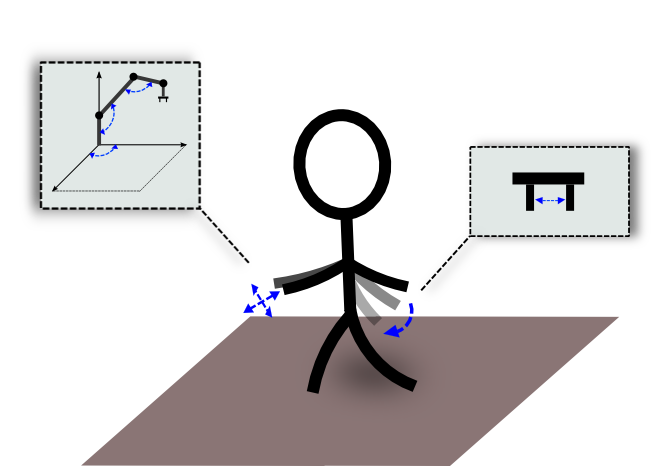
\includegraphics[scale=0.4]{imgs/singleplayer.png}
\end{center}
\end{frame}

\begin{frame}
\frametitle{Single-Player Modus}
\begin{block}{Funktionen}
\begin{itemize}
\item Rechte Hand: Steuerung von Rotation \& Beugung des Greifarms
\item Linke Hand: Öffnen/Schließen des Greifers
\item Greifer wird automatisch senkrecht zur Ebene ausgerichtet.
\end{itemize}
\end{block}

\end{frame}


\begin{frame}
\frametitle{Mulit-Player Modus}
\begin{center}
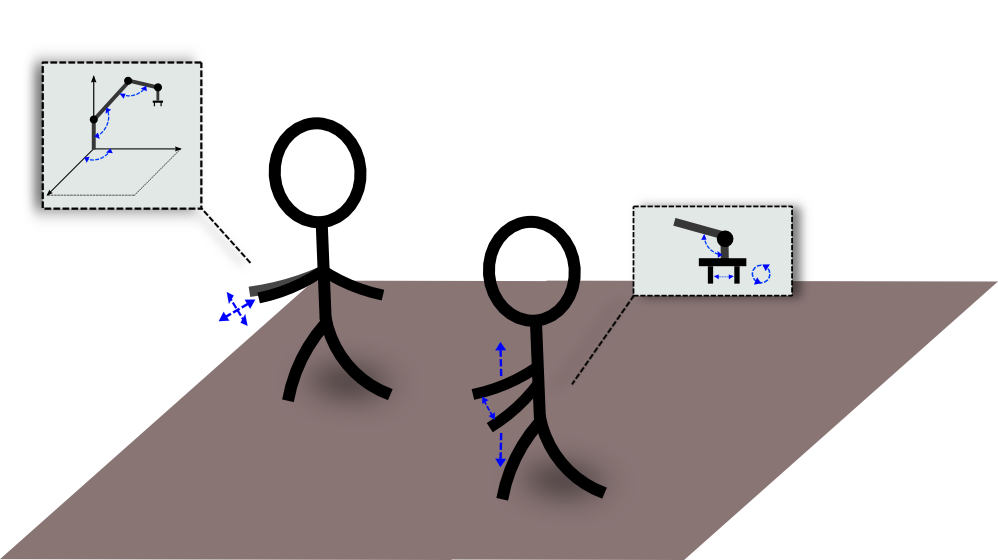
\includegraphics[scale=0.4]{imgs/multiplayer.png}
\end{center}
\end{frame}

\begin{frame}
\frametitle{Multi-Player Modus}
\begin{block}{Funktionen}
\begin{itemize}
\item 1. Spieler: Steuerung von Rotation \& Beugung des Greifarms
\item 2. Spieler: Öffnen/Schließen des Greifers
\item 2. Spieler: Rotation \& Beugung des Greifers
\end{itemize}
\end{block}
\end{frame}